\chapter{Implementation of machine learning interatomic potentials}
%\section{Modular design of MLIP}

Interatomic potential have been long time used to approximate the potential energy in classical MD simulation by a separation into separate body-order terms.
\begin{subequations}
\begin{align}
  H(\mathbf{p}, \mathbf{q}) &= \frac{\mathbf{p}^2}{2m} + V(\mathbf{q}),\\% + theromstat/barostat
  V(\mathbf{q}) &= \sum_{i = 1}^N V_1(\mathbf{q}_i) + \sum_{i,j = 1}^N V_2(\mathbf{q}_i, \mathbf{q}_j) + \sum_{i,j,k = 1}^N V_3(\mathbf{q}_i, \mathbf{q}_j, \mathbf{q}_k) + \ldots
  %\frac{\partial\mathbf{p}}{\partial t} = \frac{\partial V(\mathbf{q})}{\partial\mathbf{q}}, \\
  %\frac{\partial\mathbf{q}}{\partial t} = \frac{\partial \mathbf{p}}{m},
\end{align}
\end{subequations}
Due to limitation of hardware the first succesful approaches to interatomic potentials have been carefully handcrafted models designed for a specific materials in a specific phases.\cite{stillinger1985computer, tersoff1988empirical}.
With increased hardware power the use of data-driven models emerged allowing a more automatized model construction.
These fall under the name machine learning interatomic potentials (MLIP)\cite{bartok2010gaussian,bartok2018machine}. %TODO rather cite Behler?

The current ecosystem of ML packages is extremely abundant, that one could question why there is a need for new ML packages for the domain of material science at all.
But most of the developed packages are targeted for users that do not share the same requirements as in the domain of material science and therefore cannot be directly embedded for the development of MLIP.
This is due to the fact that the symmetrization of features based on point clouds in 3D
%symmetrized features in three-dimensional space 
 and the inference of gradients are not requirements that are shared with many other domains that deploy ML models.
To reduce the development and maintainance costs it is necessary to find points in ones method where already established software packages can be embedded in.
%This has be considered from multiple aspects does an interface happen without much loose in performance cost, is the maintainance cost of the interface lower than creating a implemantion.
For that a mathematical and algorithmic understanding of the landscape of methods and proficient skills in software development are needed which makes it such challenging problem.
%software development of MLIP remains challenging problem as most of the packages in the
%which is not a requirement that is not much shared with other domains.
%Secondly, the 
%the ML models rely on a featurization of data which is domain-dependent and therefore requires the development custom software.
%the creation of a model the shipping to an MD software.
%While featurization is domain-specific and needs custom implementations also the existing ML software ecosystem can often not to be reused for our domain as including gradients into the pictures completely changes the constraints on the required software.
%The gradient computation shifts the bottleneck drastically and thus changes the existing algorithmic design.

In this chapter I discuss my contributions to the software ecosystem that facilitates the development of MLIP.
This covers my contributions to the package \texttt{librascal} for the computation of the featurization of atomic structures and building a model, \texttt{scikit-matter} the ML method packages, implementation of an interface to \texttt{LAMMPS} that enabled study of ferroelectric phase transitions in barium titanate\cite{gigli2023modeling} as well as the transport properties of lithium ortho-thiophosphate\cite{gigli2023mechanism}.
Furthermore, this includes contributions to \texttt{equisolve} and \texttt{metatensor} that allow a more modular approach to build MLIP.

\section{Implementation of gradients in kernel models}
%As invariant 3-body descriptors are easy to evaluate from the spherical expansion coefficients without requiring additional dependencies to compute the Clebsch-Gordan coefficients as higher-body orders need and as their the memory consumption hits a sweet spot for the current generation of hardware, they have been a popular descriptor in applications.
%As their accuracy in combination with linear models is often not sufficient enough to produce accurate enough molecular dynamics simulations, one common approach has been to incorperate kernel models instead.
We do not cover an introduction to kernel methods, but only discuss the specificalities that arise when extending them for gradients.
For a comprehensive introduction to kernel models please refer to Ref.~\cite{bishop2006pattern}.

For a given kernel $k$ from a set of training samples $\{c_n\in\mathbb{R}^d\}_{t=1}^N$ and targets $\{c_n\in\mathbb{R}\}_{t=1}^N$ a set of weights $\{\alpha_n\in\mathbb{R}\}_{t=1}^N$ can be retrieved as solution of the minimization problem
\begin{subequations}
\begin{align}
  \min_\mathbf{\alpha} \sum_{n^\prime}^N\| y_{n^\prime} - \sum_{n}^N \alpha_n k(c_n, c_{n^\prime}) \|^2
\end{align}
\end{subequations}
that subsequently can be used to evaluate an arbitrary point $i$ by the relationship
\begin{equation}
  y_n = \sum_n \alpha_n k(c_n, c_i).
\end{equation}
The solution of the problem in matrix form can be expressed as
\begin{equation}
  \mathbf{\alpha} = (\mathbf{K} + \mathbf{\Lambda})^{-1}\mathbf{y}
\end{equation}
Now to include the gradients wrt. to the atomic position $\partial\mathbf{r}_k$ of atom $k$ into the picture.
We note that the training points used to construct the kernel are independent with respect to the gradients, therefore we use the notation $k_n(c_i)$ to denote $k(c_n, c_i)$ for easier readability of the derivatives
\begin{subequations}
\begin{align}
  \frac{\partial E_i}{\partial\mathbf{r}_k} &= \sum_n^N \frac{\partial \alpha_n k_n(\mathbf{c}_i)}{\partial\mathbf{r}_k} \\
    &= \sum_n^N \alpha_n \frac{k_n(\mathbf{c}_i)}{\partial\mathbf{c}_i} \frac{\partial\mathbf{c}_i}{\partial\mathbf{r}_k} \\
    &= \frac{\partial\mathbf{c}_i}{\partial\mathbf{r}_k} \sum_n^N \alpha_n \frac{k_n(\mathbf{c}_i)}{\partial\mathbf{c}_i}.
    %&= \sum_{j\in A_i}\sum_n \alpha_n \frac{k_n(\mathbf{c}_i)}{\partial\mathbf{c}_i} \frac{\partial\mathbf{c}_i}{\partial\mathbf{r}_k} \frac{\partial c_i}{\partial\mathbf{r}_k}
\end{align}
\end{subequations}
Note that the last step is is essential to reduce the number of iterations from $O(dN)$ to $O(d+N)$.
%A popular approach that works with current hardware is the sun
 % into the evaluation.
%For that reason for the work $BaTiO_3$ a kernel model was used.
Since gradients make the evaluation of the kernel matrix computationally costly, low-rank approximation techniques have become essential early on to reduce the memory intensive usage during training.
The subset of regressor method\cite{quinonero2005unifying} has been a popular low-rank estimation used in the MLIP packages \texttt{QUIP}\cite{Csanyi2007-py}.
The core idea is to project the data points on a subset of the $M$ pseudo points.
\begin{subequations}
\begin{align}
  \mathbf{K} = \mathbf{K}_{MM} + \mathbf{K}_{MN}\mathbf{\Lambda}^{-2}\mathbf{K}_{MN}^T
\end{align}
\end{subequations}
Note that to compute one kernel entry for two structures with each $N_i$ atoms it requires $N_i^2$ evaluations
\begin{subequations}
\begin{align}
  k^A(A_{i}, A_{i^\prime}) = \sum_{j\in A_i}^{N_i}\sum_{j^\prime\in A_{i^\prime}}^{N_{i^{\prime}}} k(\mathbf{c}_j, \mathbf{c}_{j^\prime}).
\end{align}
\end{subequations}
The low-rank approximation contributes greatly in the reduction of the computation of these kernel entries as it projects the structural features on single $M$ environmental features resulting in a linear scaling of on kernel entry.
Since the number of atoms in structures is a substantial quantity and the fact that structures typically contain redundant environments, the rank can be reduced quite significantly making this approach indispensable.

One disadvantage with \texttt{librascal} was the entanglement of the featurization and the model building to the libraray.
This was required as the construction of the kernel matrix requires understanding by the model building tool of the decomposition of the target property into local contributions Eq.~\ref{eq:structural_separation} as well as what its gradients are, domain-agnostic packages as \texttt{scikit-learn} are not suitable for a direct application in this case.
The software package \texttt{metatensor} allows to attribute these structural characteristics to the object itself as metadata and offers \texttt{numpy}-like data manipulations that take advantage of the metadata.
This allowed a disentanglement of the featurization that has reimplemented in a new package \texttt{rascaline} and model construction that has been moved to \texttt{equisolve}.
Part of my contribution was to participate in the development of \texttt{metatensor} as well as heavily developing on the initial design of \texttt{equisolve} contributing module of shallow methods including standardizer, linear and the above-presented kernel model as well as the inital designs for neural network models based on the data formate created in \texttt{metatensor}.
%Due to the structural nature of samples in atomistic learning, one sample consists of features for each atom presen in the structure, the  has been a popular approach as it allows a selection of individual atomic features as pseudo points unlike to the more common low-rank Nyström approach where whole structures would need to be selected.
%The partial forces in the kernel model can this be evaluated by 
%\begin{subequations}
%\begin{align}
%  E_i = \partial \sum_{j\in A_i} \sum_{t\in T} \alpha_k k(x_t, x_j) \\
%  \frac{\partial E_i}{\mathbf{r}_{ji}} = \sum_{j\in A_i} \sum_{t\in T} \alpha_k \frac{k(x_t, x_j)}{\mathbf{r}_{ji}} \\
%   \frac{k(x_t, x_j)}{\mathbf{r}_{ji}} = \frac{x_j}{\mathbf{r}_{ji}}
%\end{align}
%\end{subequations}

%Custom optimizer

%\papercomment{One could include the work on solvers here but it is note so important efficiency}

\section{Interfacing with molecular dynamics packages}
In molecular dynamics the separation of the computation of the potential energy into a separate module has been established approach\cite{LAMMPS,abraham2015gromacs,kuhne2020cp2k,kapil2019pi}.
%To make such simulations possible I implemented an interface with \texttt{LAMMPS} for our in-lab developed machine learning package \texttt{librascal} to exploit the implemented domain decomposition in \texttt{LAMMPS}.
%The correction of implementation was verified by comparing the trajectories with the MLIP package \texttt{QUIP}.
%The correctness of the interwork with LAMMPS domain decomposition was verified by running a simulation for different MPI tasks and comparing the results.
%This allowed obtain results...
As computation of the potential energy only requires the atomic positions and species and as result returns the energy with its gradients, it is a logical point to separate.
An advantage for such a separation is to avoid a reimplementation of established thermo- and barostats as well as time integrator.
While the implementation of these are in principle simple, a robust implementation that covers important corner cases still requires a longer consideration which makes it a time consuming task.
Another advantage is the fact that longly developed MD software support different parallelizations of the potential energy for interatomic potentials.
The fact that interatomic short-range potentials separate the total energy into contributions of local environments, allows a decomposition of the cell into smaller domains.
The computation of the potential energy for each of these domains can be distributed among multiple processors or machines and then be using message passing interface (MPI).
In the study of barium titanite in Ref.~\cite{gigli2023modeling} this parallelization allowed us to study the effect of long-range dielectric correlations on the predictions of the Curie temperature.
The domain decomposation requires particular considerations in the implementation of the gradients.
The force computation for an interatomic potential can be computed as
%The evaluation of gradients using the neighbor list approach is expressed
\begin{equation}
  \label{eq:forces_interatomic_potential}
  \frac{\partial E_A}{\partial\mathbf{r}_k} = \sum_{i\in A} \frac{\partial E_i}{\mathbf{r}_k} = \sum_{i\in A}\sum_{j\in A_i} \frac{\partial E_i}{\mathbf{r}_{ji}} \frac{\mathbf{r}_{ji}}{\mathbf{r}_k}\textrm{, where }\frac{\mathbf{r}_{ji}}{\mathbf{r}_k} = \begin{cases}1,& k=i \\ -1,& k=j \\0,& \textrm{ else.} \end{cases}
\end{equation}
%Without domain decomposition neighbors outside of the cell are periodic images and partial forces do not need to be assigned as they can be ignored.
%With domain decomposition neighbors outside of the cell can also be nonperiodic neighbors part of a different domain.
%\papercomment{Here I could talk about the implementation detail how to add neighbor contributions}
It can be seen that the forces at position $i$ depend on the partial forces wrt. to energy $i$ and all its neighbors $j\in A_i$.
Depending on memory storage of partial forces this case needs to be handled with care.
In particular considering the fact that MD software as \texttt{LAMMPS} offers the option to allow MPI communication between the domains with the \emph{newton\_pair} option.
Keeping the option on prevents redundant computations of the forces but requires more MPI communication as the partial forces need to be communicated.
In \texttt{librascal} if atom $j$ is a periodic neighbor, the acces on atom $j$ remapped to corresponding atom in the box.
The MPI communication requires to differ between periodic neighbors and ghost atoms that are part of another domain.
One can simplify this complexity storing the partial forces $\partial{E_i}/\partial{\mathbf{r}_{ij}}$ and $\partial{E_j}/\partial{\mathbf{r}_{ij}}$ for redundantly for atom $i$ and $j$.
This is redundant due to Netwton's third law $\partial{E_j}/\partial{\mathbf{r}_{ij}} = - \partial{E_j}/\partial{\mathbf{r}_{ji}}$.
While being redundant it does not change asympotic scaling of the memory requirements for the forces.
%i, ij
%j, ji
%i, ji
%j, ij
%where i, ij = - i, ji

\section{A metadynamic software framework with LAMMPS, PLUMED and i-PI}
To study phase transitions of barium titanite in Ref.~\cite{gigli2023modeling} we needed to accelerate the sampling of the transition.
One common technique that we use is metadynamics that adds a bias potential to the simulation that is later normalized out in the calculation of the free energy.
While the forces of the MLIP were computed with \texttt{LAMMPS} and the forces of the bias potential were computed with \texttt{PLUMED}\cite{PLUMED}.
To consolidate both forces for the metadynamics the software-package \texttt{i-PI} was used, that implemented a custom protocol to each of these MD packages to allow communicatiof the forces to a python interface.
A schematic of the interwork between the software packages can be seen in Fig.~\ref{fig:ipi-librascal-plumed}.
\begin{figure}
    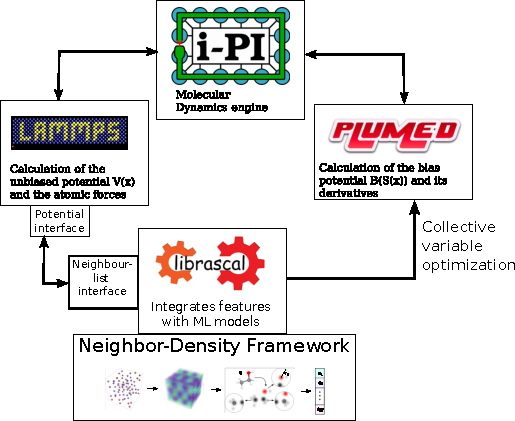
\includegraphics[width=\textwidth]{fig/ipi-librascal-plumed.pdf}
    \caption{A schematic showing the interwork of the software pieces to run metadynamic simulations to study interfacial effects of barium titanite.}
    \label{fig:ipi-librascal-plumed}
\end{figure}

As CV for the metadynamics $l=1$ components of the spherical expansion coefficients computed with \texttt{librascal} were used.
My implementation of the cubic spline helped to speed up the computation of the bias term.
Since only the expansion coefficients centered for the oxygen neighbors centered on the titanite was sufficient for the CV, I further implemented an option to selectively computate the partial gradients for certain species.
Note that a selectional computation of partial gradients also needs to consider dependencies of the gradient on the central energies of its neighbors as pointed out in Eq.~\ref{eq:forces_interatomic_potential}.
%implementation of was implemented by me to speed up the metadynamics simulation
%work are adjustments to the
%In the subsequent sections we will discuss the technica
%My contributions to this work was firstly, to participate in the development of the MLIP package \texttt{librascal} that was used to conduct DFT simulations at higher levels-of-theory to analyse its effect on the temperature.
%Specifically, the implementation of selective computations of the partial gradients for certain species was implemented by me to speed up the metadynamics simulation.
%Secondly, the implementation of an interface to the MD software \texttt{LAMMPS} that allowed to study the finite size effects on the Curie temperature.

%The interface was implemented by Gareth Tribello.

%\section{Modular design of MLIP}
%As scientific methods continue to evolve, the demands placed on software to incorporate these advancements also grow.
%%While advances in methodolgy can prove to improve a method in all aspects, and thus replace an existing method, it is more often the case that they extend the capabilities and requiring more flexibility of the software outside of the initial design of the software package.
%While improvements in method development often lead to enhanced efficiency and user-friendliness, they typically extend the software's capabilities beyond its original design.
%As software is extended by more features over time, it tends to become less adaptable to changes to incorperate newly developed methods.
%Consequently, rapid advancements in methodology can render software obsolete before the development is even at the stage of deployment for experiments.
%%Considering that software becomes more rigid to changes over time with increased number of implemented features, it is a natural consequence that with a rapid development in methodology the software becomes deprecated as it cannot keep up with these changes.
%Similar challenges were observed in the 1960s when rapid hardware development contributed to a software crisis\cite{brian2012software_crisis}.
%However, as development progresses, also the understanding of critical components for performance emerges which solidifies the possible software designs to retrieve performant code.
%With this places in the software naturally appear that can be used to decompose it into separate components allowing to distribute the software development workload among peers.
%%groups as they can independently work on the individual modules.
%This not only allows to speed up the development but it also allows a more specialized development leading to more performant code.
%While scientific publications cover abundantly method development based on mathematical advancements, the modular design of software implementing a variety of methods in a specific domain is still highly underrepresented in the scientific literature even though it dictates the efficiency the method development.
%%With regard to incensitives present academia that only fund software development tied to new scientific applications, the existing fragmented landscape of unmaintained monolothic software packages solving over and over again the same problem is a natural consequence.
%%Advances can be only made when enough money is allocated to a group that recognizes the need to create a software package standardizing interfaces.
%This section discusses modular design patterns relevant for the domain of atomistic learning to integrate of machine learning interatomic potentials with molecular dynamics packages.
%Interfaces where applicable are needed to reduce software costs for groups focusing on optimization of .
%Modular design is essential for sustainable scientific problem: Not reinventing the wheel, extensibility, wider-applicability, focused problem-solving
%The production of reliable and maintained software is essential for the progress of further scientific development to  prevent a scientfic crisis as in the \cite{TODO}.
%
%%\section{MLIP}
%%A common approach for the integration of machine learning into the molecular dynamics simulation
%%\begin{equation}
%%  H(\mathbf{p}, \mathbf{q}) = \frac{\mathbf{p}^2}{2m} + V(\mathbf{q})% + theromstat/barostat
%%\end{equation}

%Note that contributions to the gradient come from the partial gradients $\partial E_k/\mathbf{r}_{jk}$ 
%wrt. to the distance vector to all neighbors 
%\emph{and} from $\partial E_j/\mathbf{r}_{kj}$ where $j$ is in the neighborhood of atom $k$ ($j\in A_k$). 
%additional pr to be done to allow contiguous iteration during the computation of the gradients.

%Note that one can simplify the gradients for further usage by summing neighbour and central contributions
%\begin{subequations}
%\begin{align}
%  \mathbf{F}_{kj} = -\frac{\partial E_k}{\mathbf{r}_{jk}} + \frac{\partial E_j}{\mathbf{r}_{kj}} \\
%  \frac{\partial E_A}{\partial\mathbf{r}_k} = \sum_{j\in A_k} \mathbf{F}_{kj}.
%\end{align}
%\end{subequations}

%\cite{https://docs.lammps.org/Developer_write_pair.html}
%As classical molecular dynamics simulation require the computation

%In this section we will discuss the approach that is taken in software for classical molecular dynamics code as \cite{LAMMPS, Gromacs, CP2K, Plumed, Jaxmd, OpenMMTODO}.
%%equilibrium hat uses the Born-Oppenheimer approximation 
%%software simulating equilibrium dynamics using the Born-Oppenheimer approximation so 
%%equilibrium hat uses the Born-Oppenheimer approximation 
%%A common approach for equilibrium molecular dynamics software is to 
%From the equations of motion 
%\begin{subequations}
%\begin{align}
%  H(\mathbf{p}, \mathbf{q}) = \frac{\mathbf{p}^2}{2m} + V(\mathbf{q}),\\% + theromstat/barostat
%  \frac{\partial\mathbf{p}}{\partial t} = \frac{\partial V(\mathbf{q})}{\partial\mathbf{q}}, \\
%  \frac{\partial\mathbf{q}}{\partial t} = \frac{\partial \mathbf{p}}{m},
%\end{align}
%\end{subequation}
%we obtain 
%a separation of the computation of kinetic and potential energy into separated modules arises.
%Depending on the type of thermodynamic ensemble and subsequently the thermo- or barostat the kinetic energy and its derivative, the differently evaluated.
% TODO I don't know if these are really easy changes
%As the evaluation of the kinetic energy, even considering the correction by thermo- or barostat, is computationally not significant, a lot of method development and specialized software has been focused on making the evaluation of the potenial energy more efficient.

%The potential energy can be further separated into a short- and long-range term
%\begin{equation}
%  V(\mathbf{q}) = V_\textrm{short}(\mathbf{q}) + V_\textrm{long}(\mathbf{q}).
%\end{equation}
%Often MD software separate the calculation of both parts into separate module as $V_\textrm{short}$ is computed in real space and the $V_\textrm{long}(\mathbf{q})$ typically is computed in Fourier space as much is not reused thus not much can be recomputed.
%Therefore both require different types of data structures  and resolved in complicated 
%and therefore the separation into separate modules naturally arises.
%
%take computationally advantage of using a neighborlist using binning (also known as voxel) algorithms\cite{TODO} while the long-range part can be computationally efficient evaluated in Fourier space using partical mesh methods\cite{TODO}.
%Under the assumption of uniformly distributed system the theoretical complexity is $O(N\log N)$ instead of $O(N^2)$ in the implementation of naive scaling.
%Even though a perfect uniform distribution is almost never fulfilled for a system, it is reasonable to assume one is close enough to such a state for a large part of the states during a simulation that the theoretical scaling is approximative true.
%Note that theoretical scaling arguments completely ignore constant overheads due to preprocessing or improvements due to hardware capacities (e.g. cache locallity, hardware capability of parallel processing) that are essential for real applications. 

%MPI pair contributions of forces requiring reorganisation of contributions to consider ghost neighbors correctly.
%One advantage for such a separation is that the implementation of the thermo- and barostats different ensembles, the calculation of the neighborlist can be separated in different parts of the code.
%optimization of the calculation of the neighborlist can be separately
%An advantage of the development of software dedicated for the creation of interatomic potentials separate from the other parts of the MD software.
%The parts that control how the MD work thus do not need be reimplemented and optimizations of the neighborlist with MPI can be reused.
%A disadvantage of the modularity can be seen in example for a long-range potential.
%While usually 

%\subsection{Application LAMMPS Plumed interface for interfacial effects on BaTiO3}

%\section{Modularity in MLIP}
%There are several things we learn from technical analysis details that prevent a modular design as present it exists for traditional machine learning algorithms.
%Narative:
%An essential prevention for modularity is that the computation of the kernel requires a sparse data format hash mappable due to the species polynomial growth
%Secondly, most ML packages do not support gradients in their methodology.
%A recent develompent.

%\subsection{MLIP interface}

\section{Serialization of MLIP}
In last decade, the rapid development of machine learning models has resulted in numerous interfaces for \texttt{LAMMPS}\cite{QUIP}. %TODO more
While the model accuracy is a good indicator for the usability of a model, it is still not reliable enough to be a guarantee that the model will work for MD software as undersampling of the phase space can always be an issue for any kind of model.
One is therefore forced to retrain the model for a dataset covering a larger part of the phase pace or switch to a more accurate model during the analysis of an experiment.
As all ML models show different trade-offs between accuracy, evaluation time, trainings cost and hyperparameter optimization the set of suitable models depend on the system of interest, the dataset size and given computational resources.
As the dataset size changes over the course of analysis different models become more suitable candidates and thus a different model is more suitable for the analysis.
%It has been shown that linear models can be competetive in high data regime. %TODO verify that
The current software infrastructure of ML models for MD software causes a lot of friction when changing the model type as the MD software needs to be recompiled for a different interface.% and a new workflow pipeline has to be constructed.
Even more crucial is the fact that the model development is often conducted in higher-level languages like \texttt{Python} or \texttt{Julia} due to their flexibility.
This however restricts the usage of the model also to MD packages in the same higher-level langue or requires the implementation of a serialization for the model plus interface for an MD package.
This work restricts the usage of a lot of developed ML models in low-level MD packages which are often required to conduct insightful research.
For nearly five years following its initial publication, the widely-used SchNet model\cite{schu+18jcp} lacked an interface with a low-level MD package.
%This however restricts the usage of the model also to higher-level when no serialization exists. 
%Heteregoneous hardware optimizer: OneAPI, Kokkos
Similar problems exists in industry where models trained with different ML packages need to be shipped to devices with different hardware architectures and different software stacks making it hard to reliably provide the same version of the package on each device.
The industry therefore developed an open standard for machine learning models open neural network exchange (ONNX).
This standard can however not be used for MLIPs as they lack the support of the inference for gradients.
%Since the majority of ML models are constructed in higher-level languages, most MD engines are written in a low-level language for performance reasons.
%It is thus needed to export models to a standardized formate that allows to execute models in the low-level languaes
%Low-level language for efficiency, scripting-like for flexibility

%to export models to one software from memory to disk for reproducibility and hardware independency (e.g. JSON).

The Open Knowledgebase of Interatomic Models (OpenKIM)\cite{karls2020openkim} tries to address the problem.
They developed abstract representations of the data and processing directives necessary to perform a molecular simulation thereby unifying the interfaces of several MD packages to one interface, namely the KIM API\cite{elliott2011kim}.
While it reduces the cost of the number interfaces that are needed, they are far from covering comprehensively all relevant MD packages, as packages like GROMACS\cite{hess+08jctc} and C2PK\cite{kuhne2020cp2k} are missing.
Most of the supported MD packages are implemented in higher-level languages for which a custom MLIP interface can be easily implemented.

A solution we target with the software ecosystem developed in our lab is to use TorchScript as it supports the use of gradients and offers a usage of the model in C++ surpassing the high-level language barrier.
It further supports advances model optimization utilities that can be used optimize complex models by kernel fusioning of the operation graph.
Considering all that it seems like a promising candidate to standardize the landscape of MLIPs.

%\section{Foreign-Function interface [optional]}
%Low-level language for efficiency, scripting-like for flexibility
%Libraries that https://www.swig.org/compat.html
%Check out \url{https://docs.rs/rust_swig/latest/rust_swig/#enums}
%However these are not working with TorchScript, also Julia is missing that is becoming essential for scientific softwared development

%\section{Machine learning ecosystems}
%
%\subsection{Hardware kernels}
%\subsection{scikit-learn - close-form inspired infrastructure}
%- transformers, models
%- fit function needs to be specified that optimizes one object
%- concatenation of models through Pipelines allows parameter optimization over different modules however it is every rigid (sample dimension cannot change over the pipelines)
%\subsection{torch - autograd inspired infrastructure}
%Dataloader:
%- concatenation of indicies
%- caching
%Optimizer:
%- concatenation of indicies
%- caching
%While torch summarizes all existing optimizers under one library, Jax approaches this issue with modularity\cite{jaxopt_implicit_diff}
%\subsection{Standardization array-APIs}
%mention Array-API
%https://data-apis.org/array-api/latest/

%\section{MLIP for applications on ferroelectrics}
%\section{Metadynamic framework using MLIP}
%We have seen development of splining algorithms.
%In the chapter we cover a specific application where this supported the work
%
%A ferroelectric is a material that possesses a permanent electric polarization that can be switched under the action of an external electric field.
%Typically, the emergence of the polar phase is accompanied by a structural transition from a high-symmetry paraelectric state down to a broken-symmetry state with a characteristic long-range dipolar ordering [1, 2].
%Early studies on ferroelectrics using ab-initio calcluation [23, 24] have identified discrepancies between the temperatures at which structural transitions occur in the simulations and the temperatures at which these transitions occur in reality.
%These discrepancies are often reduced by introducing artificial corrections to the simulated pressure [25–27].
%This additional pressure brings the simulation volume closer to the values seen in experiments and drives the predicted Curie temperature towards its experimental value.
%However, this correction tells us little about the physical origins for the discrepancies that are observed in simulations.
%There are multiple sources of error that could be the origin for these discrepancies.
%(1) The GGA functional (PBEsol) [28] used in previous work slightly underestimates the equilibrium volume of cubic BaTiO3.
%(2) The determination of the transition temperature by tracking spontaneous fluctuations between the phases limits the system size that can be studied, despite the reduced computational cost of the ML potential.
%The paraelectric-ferroelectric phase transition needs to be therefore studied by using metadynamics simulations.
%
%%work are adjustments to the
%%In the subsequent sections we will discuss the technica
%%My contributions to this work was firstly, to participate in the development of the MLIP package \texttt{librascal} that was used to conduct DFT simulations at higher levels-of-theory to analyse its effect on the temperature.
%%Specifically, the implementation of selective computations of the partial gradients for certain species was implemented by me to speed up the metadynamics simulation.
%%Secondly, the implementation of an interface to the MD software \texttt{LAMMPS} that allowed to study the finite size effects on the Curie temperature.
%
%To conduct metadynamics a bias term based on the spherical expansion coefficients was computed \texttt{PLUMED} using \texttt{librascal}
%%The interface was implemented by Gareth Tribello.
%To consolidate the forces computed with \texttt{LAMMPS} and the bias term computed with \texttt{PLUMED} to run metadynamics the software-package \texttt{i-PI} was used, that implemented a custom protocol to each of these packages to allow communication betwe.
%A schematic of the interwork between the software packages can be seen in Fig.~\ref{fig:ipi-librascal-plumed}.
%\begin{figure}
%    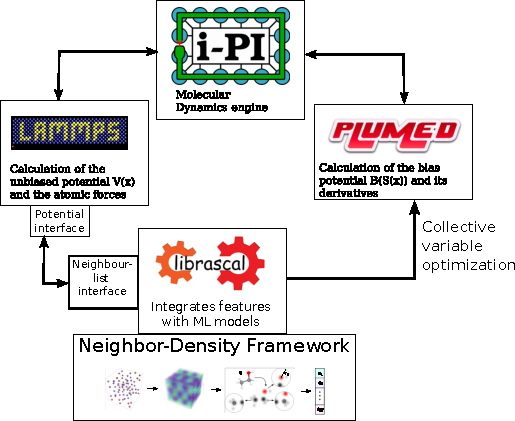
\includegraphics[width=\textwidth]{fig/ipi-librascal-plumed.pdf}
%    \caption{A schematic showing the interwork of the software pieces to run metadynamic simulations to study interfacial effects of $BaTiO_3$.}
%    \label{fig:ipi-librascal-plumed}
%\end{figure}
